\documentclass[12pt]{extarticle}

\usepackage{graphicx}

\title{
{\LARGE \bfseries Predicting the Upcoming Primaries using Twitter Data}
}

\author{Scott Sullivan}

\begin{document}

\maketitle

\newpage

\section{Introduction}
Twitter offers a valuable source of data for analyzing political sentiment among potential voters.
The popularity of political discussions on Twitter makes it possible to aggregate large datasets in a relatively short time.
The sheer volume of data makes it possible to calculate statistics for many state-candidate combinations with reasonably small statistical uncertainties.
By averaging statistical trends across different regions, it should be possible to reduce statistical biases and make accurate predictions.
\\
\indent
The goal of this paper was to analyze the predictive power of Twitter in the context of the democratic primary elections.
The main questions addressed were:
\begin{enumerate}
\item To what degree can Twitter data ascertain the underlying voter sentiment for each candidate?
\item How consistent are the statistics across state boundaries?
\item How well can these data be used to predict the upcoming primary results?
\end{enumerate}
The methods for downloading tweets, calculating statistics, and estimating uncertainties are explained in section 2.
The statistics from past elections and predictions for future elections are presented in section 3.
The main trends and conclusions are highlighted in section 4.

\section{Methods}
The data analysis pipeline is explained below.
First Twitter users were classified according to their state and supported candidate.
Next, for past primaries in each state, ratios were calculated which relate Twitter support to real votes.
Finally, these ratios were averaged and used to predict future primaries.
\subsection{Downloading and Classifying Tweets}
First, tweets were downloaded and classified as either pro-Sanders or pro-Clinton.
Rather than using sentiment analysis, each tweet was filtered using hashtags.
The advantage of hashtags is that the sentiment of each tweet is unambiguous.
For instance, a tweet containing \texttt{\#feelthebern} is overwhelmingly likely to be pro-Sanders, while \texttt{\#imwithher} is overwhelmingly likely to be pro-Hillary.
The only disadvantage is less data, as many relevant tweets are excluded because they don't contain the prescribed hashtags.
The hashtags used in the analysis are shown in the table below.
\\
\\
\begin{centering}
	\begin{tabular}{|c|c|} \hline
    Candidate & Positive hashtags \\ \hline 
		Bernie Sanders & \texttt{\#feelthebern}, \texttt{\#bernieorbust}, \texttt{\#stillsanders}, \texttt{\#bernie2016} \\ \hline
		Hillary Clinton & \texttt{\#hillary2016}, \texttt{\#imwithher}, \texttt{\#clintonfoundation} \\ \hline
  \end{tabular}
\end{centering}
\\
\\
For the analysis, estimates for candidate support were based on number of users rather than number of tweets.
This removes any bias towards users who tweet more often and reflects the fact that each user can only vote once.
Each user's preferred candidate was calculated by tallying their pro-Clinton tweets versus pro-Sanders tweets and taking the greater of the two.
\\
\indent
Next, users were classified into different states.
Matching a simple regular expression on each user's location could reliably retrieve a user's state for about a third of all users.
The algorithm matched either the state's full name, or the state's abbreviation if it was at the end.
For Washington, the full-name match was excluded in order to avoid ambiguity with the District of Columbia.

\subsection{Relating Twitter support to voter support}
The main goal was to calculate a statistic that was consistent across state boundaries.
The statistic should directly relate Twitter supporters to voters in each past primary in order to predict future primaries.
For the 44 states whose primary has already occured, the number of votes for each candidate was downloaded from Google and compared with the number of Twitter supporters.
A ratio was chosen in such a way as to reduce known biases while quantifying the uncertainty from unknown biases.
\\
\indent
The first known bias resulted from confounding variables between each candidate's Twitter supporters and actual voters.
For example, if Sanders supporters are younger, and Twitter users are also younger, than Sanders would be overestimated in the Twitter data relative to the election results.
To take this bias into account, the ratio between primary voters and Twitter supporters was calculated for each state and candidate combination.
If $V_S$ was the number of Sanders voters in a state, and $T_S$ was the number of Sanders Twitter supporters in a state, the ratio $R_S = V_S / T_S$ can be defined as the ratio between voters and Twitter supporters.
Similarly, $R_C$ can be defined for Clinton as the ratio between Clinton voters and Clinton Twitter supporters in a state.
\\
\indent
The second bias was the varying degree of total voters in each state for past primaries.
Some states had caucuses, others had closed primaries, and others had open primaries.
The different rules in each state created large fluctuations in the total amount of voter participation, which in turn created large fluctuations in $R_S$ and $R_C$.
Therefore, simply averaging $R_S$ and $R_C$ across states was not feasible.
However, a new ratio was defined as $R_R = R_S / R_C$.
This ratio of ratios should be similar across all states, since it is independent of total voter participation.
The ratio of ratios can be fitted by averaging data from past primaries, then be used to predict future primaries.
\\
\indent
It should be noted that when averaging $R_R$, a geometric mean was used as opposed to an arithmetic mean.
This was to preserve the symmetry between swapping the numerator (Sanders) and denominator (Clinton) of $R_R$.
We expect that $\langle R_S/R_C \rangle = 1 / \langle R_C/R_S \rangle$, which is a property that holds for geometric means.
\\
\indent
If the ratio of ratios $R_R$ is fitted from past primaries, and the number of Twitter supporters for each candidate is known for future primary states, then the number of predicted delegates can be estimated as follows.
The ratio of votes is given by
\begin{equation}
\frac{V_S}{V_C} = \frac{R_S T_S}{R_C T_C} = R_R \frac{T_S}{T_C}.
\end{equation}
This should be proportional to the ratio of delegates,
\begin{equation}
\frac{D_S}{D_C} = R_R \frac{T_S}{T_C}.
\end{equation}
Let D be the number of delegates in a state whose primary has not happened yet.
By normalizing with $D_S + D_C = D$, we can predict the number of delegates obtained by each candidate.
Let $x = D_S / D_C$.
The estimated delegates are given by
\begin{equation}
	\label{eq:ds}
D_S = \frac{x}{1+x} D,
\end{equation}
\begin{equation}
	\label{eq:dc}
D_C = \frac{1}{1+x} D.
\end{equation}

\subsection{Estimating Uncertainties}
To estimate uncertainties, the count of Twitter users from each state was assumed to come from a Poisson distribution.
Therefore, the uncertainties in $T_S$ and $T_C$ were $\sigma_{T_S} = \sqrt{T_S}$ and $\sigma_{T_C} = \sqrt{T_C}$, respectively.
For each state, the uncertainties in $R_S$ and $R_C$ were propagated using partial derivatives,
\begin{equation}
	\sigma_{R_S} = \frac{R_S}{V_S} \sigma_{V_S}.
\end{equation}
\begin{equation}
	\sigma_{R_C} = \frac{R_C}{V_C} \sigma_{V_C}.
\end{equation}
The uncertainties for each state's ratio of ratios were propagated using partial derivatives,
\begin{equation}
	\sigma_{R_R} = \sqrt{\Big(\frac{R_R}{R_S} \sigma_{R_S}\Big)^2 + \Big(\frac{R_R}{R_C} \sigma_{R_C}\Big)^2}.
\end{equation}
The average value for $R_R$ was calculated using a weighted geometric mean, where the weights came from different uncertainties in each state.
The geometric mean and uncertainty were calculated using three steps:
\begin{enumerate}
	\item For each state $i$, take the log of the ratio,
		\begin{equation}
		y_i = \log{R_{R_i}},
	\end{equation}
	\begin{equation}
		\sigma_{y_i} = \frac{1}{R_{R_i}} \sigma_{R_{R_i}},
	\end{equation}

	\item For each state $i$, calculate the weighted mean and weighted variance in log-space,
		\begin{equation}
			\langle y \rangle = \frac{\sum_i w_i y_i}{\sum_i w_i},
		\end{equation}
		\begin{equation}
			\sigma_{\langle y \rangle}^2 = \frac{1}{\sum_i w_i} \frac{1}{N-1} \sum_i w_i \Big(y_i - \langle y \rangle \Big)^2,
		\end{equation}
		\begin{equation}
			w_i = \frac{1}{\sigma_{y_i}^2}
		\end{equation}
	\item Return to normal space using
		\begin{equation}
			\langle R_R \rangle = e^{\langle y \rangle},
		\end{equation}
		\begin{equation}
			\sigma_{\langle R_R \rangle} = e^{\langle y \rangle} \sigma_{\langle y \rangle}.
		\end{equation}
\end{enumerate}
The uncertainty was derived from the standard deviation, as opposed to the standard deviation of the mean.
This was because each future primary should be expected to follow the same spread as past primaries.
\\
\indent
Finally, the uncertainty in future states was a combination of Poisson error from each state's count of Twitter users and the uncertainty in $R_R$.
Recalling the definition of $x = T_S / T_C$, the uncertainty in $x$ is given by
\begin{equation}
	\sigma_x = \sqrt{\Big(\frac{x}{T_C} \sigma_{T_C}\Big)^2 + \Big(\frac{x}{T_S} \sigma_{T_S}\Big)^2}.
\end{equation}
For each candidate, the delegate uncertainty propagates from equations \ref{eq:ds} and \ref{eq:dc},
\begin{equation}
	\sigma_{D_S} = \frac{D_S}{(1+x)^2} \sigma_x,
\end{equation}
\begin{equation}
	\sigma_{D_C} = \frac{D_C}{(1+x)^2} \sigma_x.
\end{equation}

\section{Results}
Tweets were accumulated over a period of about ten hours, resulting in 40,500 relevant tweets and 5,000 unique users.
Typically there were 50 users per candidate per state, so Poisson errors were on the order of 10-20\%.
\\
\indent
The average ratio of ratios was given by
\begin{equation}
R_R = 0.57 \pm 0.06.
\end{equation}
This number essentially tells us Sanders' overrepresentation on Twitter.
For every matching primary vote between Sanders and Clinton, there should be a ratio of roughly five-to-three of Sanders over Clinton on Twitter.
For an understanding of how these ratios vary across states, $R_R$ for each state is shown in figure \ref{fig:rr}.
\begin{figure}
\centering
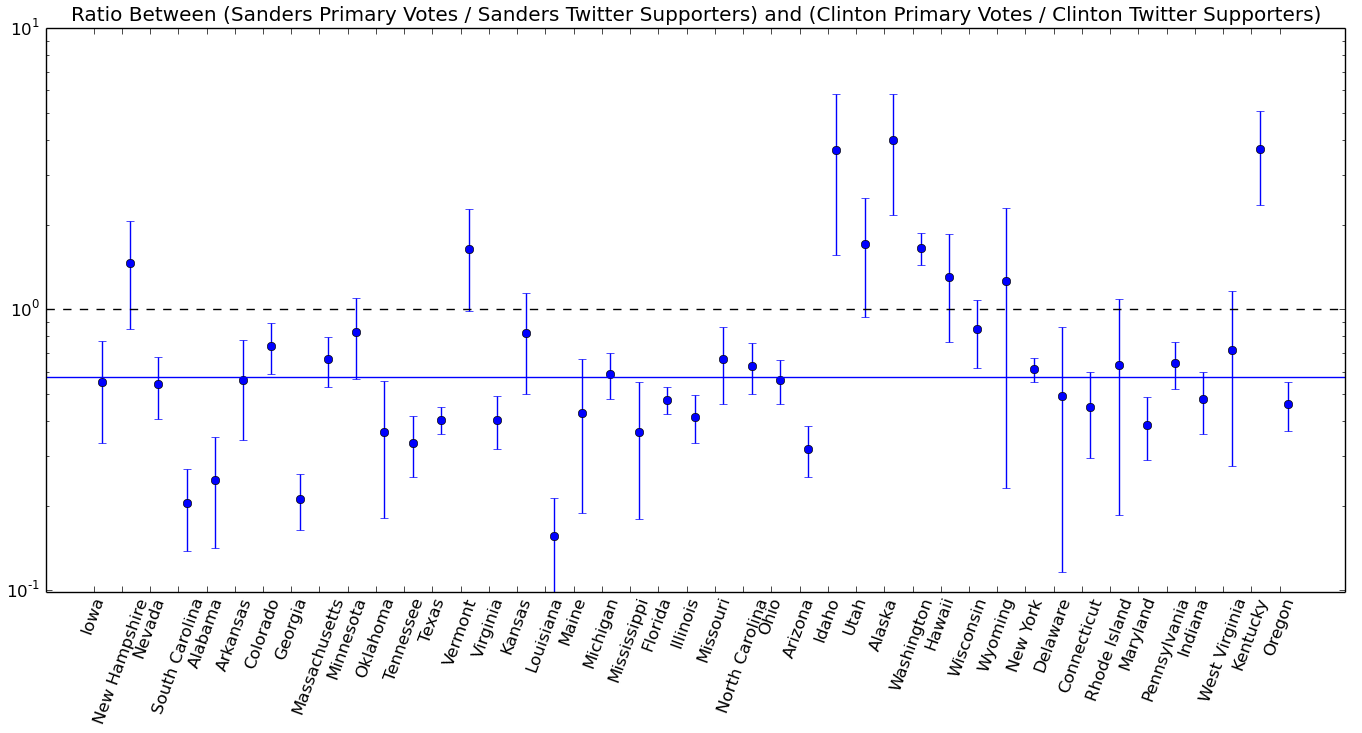
\includegraphics[width=\linewidth]{ratio_ratios.png}
\caption{$R_R$ by state. The uncertainties were from assuming a Poisson distribution when counting Twitter users.}
\label{fig:rr}
\end{figure}
\\
\indent
Information for the predicted results are shown in the tables below.
South Dakota was excluded for not having any Clinton Twitter supporters.
First are the Twitter supporters in the five remaining states.
\\
\\
\begin{centering}
  \begin{tabular}{|l|l|l|}
	  \hline
     State & Sanders Twitter supporters & Clinton Twitter supporters \\
	  \hline
	  \hline
     North Dakota & 4 & 2 \\
     California & 855 & 250 \\
     New Jersey & 67 & 44 \\
     New Mexico & 23 & 10 \\
     Montana & 13 & 2 \\
	  \hline
  \end{tabular}
\end{centering}
\\
\\

Next are the expected delegates in each state.
\\
\\
\begin{centering}
	\begin{tabular}{|l|l|l|l|l|}
	  \hline
  State & Sanders Delegates & Uncertainty & Clinton Delegates & Uncertainty \\
	  \hline
	  \hline
  North Dakota & 9 & 2 & 8 & 1 \\
  California & 314 & 29 & 160 & 16 \\
     New Jersey & 59 & 8 & 67 & 7 \\
     New Mexico & 19 & 5 & 15 & 3 \\
     Montana & 17 & 4 & 4 & 1 \\
	  \hline
  \end{tabular}
\end{centering}
\\
\\
Finally are the total delegates from the five states.
\\
\\
\begin{centering}
	\begin{tabular}{|l|l|l|l|l|}
	  \hline
	  Candidate & Total Delegates & Uncertainty \\
	  \hline
	  \hline
	  Bernie Sanders & 481 & 31 \\
	  \hline
	  Hillary Clinton & 256 & 18 \\
	  \hline
  \end{tabular}
\end{centering}
\\
\\
\section{Conclusion}
By calculating a ratio of ratios, $R_R = R_S / R_C$, a number of biases were removed.
However, figure \ref{fig:rr} shows that many state ratios still lie well outside their error-bounds.
This is likely due to unaccounted biases across different states.
But even with unaccounted biases, the spread is still small enough to warrant a prediction for future primaries.
\\
\indent
According to this model, we should expect Sanders to win California by a significant margin, roughly 150 delegates.
Sanders should also win North Dakota and Montana, although the number of counted Twitter users is small enough that an upset wouldn't be surprising.
Clinton has a slight lead in New Jersey, while Sanders has a slight lead in New Mexico.
Currently Sanders is behind by about 290 delegates, and could catch up by as much as 230 delegates during the June 7 primaries.
While this is not enough to overtake Clinton in pledged delegates, it does approach the uncertainty estimates.
An upset would be unlikely, but not completely out-of-the-question.
\\
\indent
It would be interesting to attempt a similar analysis in the general election.
This particular analysis exploited the spaced timings of past primaries, which allowed fitting past statistics to cast predictions.
This feature unfortunately is not available in the general election.
However, perhaps votes in past Republican primaries could be used to fit ratios which could be reused in the general election.

\end{document}
